\documentclass[a4paper]{article}
\usepackage{geometry}
\usepackage{graphicx}
\usepackage{natbib}
\usepackage{amsmath}
\usepackage{amssymb}
\usepackage{amsthm}
\usepackage{paralist}
\usepackage{epstopdf}
\usepackage{tabularx}
\usepackage{longtable}
\usepackage{multirow}
\usepackage{multicol}
\usepackage[hidelinks]{hyperref}
\usepackage{fancyvrb}
\usepackage{algorithm}
\usepackage{algorithmic}
\usepackage{float}
\usepackage{paralist}
\usepackage[svgname]{xcolor}
\usepackage{enumerate}
\usepackage{array}
\usepackage{times}
\usepackage{url}
\usepackage{fancyhdr}
\usepackage{comment}
\usepackage{environ}
\usepackage{times}
\usepackage{textcomp}
\usepackage{caption}


\urlstyle{rm}

\setlength\parindent{0pt} % Removes all indentation from paragraphs
\theoremstyle{definition}
\newtheorem{definition}{Definition}[]
\newtheorem{conjecture}{Conjecture}[]
\newtheorem{example}{Example}[]
\newtheorem{theorem}{Theorem}[]
\newtheorem{lemma}{Lemma}
\newtheorem{proposition}{Proposition}
\newtheorem{corollary}{Corollary}

\floatname{algorithm}{Procedure}
\renewcommand{\algorithmicrequire}{\textbf{Input:}}
\renewcommand{\algorithmicensure}{\textbf{Output:}}
\newcommand{\abs}[1]{\lvert#1\rvert}
\newcommand{\norm}[1]{\lVert#1\rVert}
\newcommand{\RR}{\mathbb{R}}
\newcommand{\CC}{\mathbb{C}}
\newcommand{\Nat}{\mathbb{N}}
\newcommand{\br}[1]{\{#1\}}
\DeclareMathOperator*{\argmin}{arg\,min}
\DeclareMathOperator*{\argmax}{arg\,max}
\renewcommand{\qedsymbol}{$\blacksquare$}

\definecolor{dkgreen}{rgb}{0,0.6,0}
\definecolor{gray}{rgb}{0.5,0.5,0.5}
\definecolor{mauve}{rgb}{0.58,0,0.82}

\newcommand{\Var}{\mathrm{Var}}
\newcommand{\Cov}{\mathrm{Cov}}

\newcommand{\vc}[1]{\boldsymbol{#1}}
\newcommand{\xv}{\vc{x}}
\newcommand{\Sigmav}{\vc{\Sigma}}
\newcommand{\alphav}{\vc{\alpha}}
\newcommand{\muv}{\vc{\mu}}

\newcommand{\red}[1]{\textcolor{red}{#1}}

\def\x{\mathbf x}
\def\y{\mathbf y}
\def\w{\mathbf w}
\def\v{\mathbf v}
\def\E{\mathbb E}
\def\V{\mathbb V}

% TO SHOW SOLUTIONS, include following (else comment out):
\newenvironment{soln}{
	\leavevmode\color{blue}\ignorespaces
}{}


\hypersetup{
	%    colorlinks,
	linkcolor={red!50!black},
	citecolor={blue!50!black},
	urlcolor={blue!80!black}
}

\geometry{
	top=1in,            % <-- you want to adjust this
	inner=1in,
	outer=1in,
	bottom=1in,
	headheight=3em,       % <-- and this
	headsep=2em,          % <-- and this
	footskip=3em,
}


\pagestyle{fancyplain}
\lhead{\fancyplain{}{Homework 1}}
\rhead{\fancyplain{}{CS 760 Machine Learning}}
\cfoot{\thepage}

\title{\textsc{Homework 1}} % Title

%%% NOTE:  Replace 'NAME HERE' etc., and delete any "\red{}" wrappers (so it won't show up as red)

\author{
	{RYAN YEE} \\
	{9074025223}\\
} 

\date{}

\begin{document}
	
	\maketitle 
	
	
	\textbf{Instructions:} 
	This is a background self-test on the type of math we will encounter in class. If you find many questions intimidating, we suggest you drop 760 and take it again in the future when you are more prepared.
	
	Use this latex file as a template to develop your homework.
	Submit your homework on time as a single pdf file to Canvas.
	There is no need to submit the latex source or any code.
	Please check Piazza for updates about the homework.
	
	
	\section{Vectors and Matrices [6 pts]}
	Consider the matrix $X$ and the vectors $\mathbf{y}$ and $\textbf{z}$ below:
	$$
	X = \begin{pmatrix}
		3 & 2 \\ -7 & -5 \\
	\end{pmatrix}
	\qquad \mathbf{y} = \begin{pmatrix}
		2 \\ 1
	\end{pmatrix} \qquad \mathbf{z} = \begin{pmatrix}
		1 \\ -1
	\end{pmatrix}
	$$
	\begin{enumerate}
		\item 	Computer $\mathbf{y}^{T} X \mathbf{z}$\\
			    \begin{soln} 
					$$
					\begin{aligned}
						\mathbf{y}^{T} X \mathbf{z} & = \begin{pmatrix} 2 & 1 \end{pmatrix} \begin{pmatrix} 3 & 2 \\ -7 & -5 \\ \end{pmatrix} \begin{pmatrix} 1 \\ -1 \end{pmatrix} \\
						& = \begin{pmatrix} 2 & 1 \end{pmatrix} \begin{pmatrix} 1 \\ -2 \end{pmatrix} \\
						& = 0 
					\end{aligned}
					$$
				\end{soln}
		\item 	Is $X$ invertible? If so, give the inverse, and if no, explain why not.\\
		        \begin{soln}
					$$
					\begin{aligned}
						X^{-1} & = \frac{1}{-1} \begin{pmatrix} -5 & -2 \\ 7 & 3 \end{pmatrix} \\
						& = \begin{pmatrix} 5 & 2 \\ -7 & -3 \end{pmatrix} 
					\end{aligned}
					$$
				\end{soln}
	\end{enumerate}
	
	
	\section{Calculus [3 pts]}
	\begin{enumerate}
		\item If $y = e^{-x} + \arctan(z)x^{6/z} - \ln\cfrac{x}{x+1}$, what is the partial derivative of $y$ with respect to $x$?\\
		\begin{soln} 
			$$
			\begin{aligned}
				\frac{\partial y}{\partial x} & = -e^{-x} + \frac{6}{z} \arctan(z) x^{(6/z) - 1} - \frac{x+1}{x} \left(\frac{(x+1)-x}{(x+1)^{2}}\right) \\
				& = -e^{-x} + \frac{6}{z} \arctan(z) x^{(6/z) - 1} - \frac{1}{x(x+1)} 
			\end{aligned}
			$$
		\end{soln}
	\end{enumerate}
	
	
	\section{Probability and Statistics [10 pts]}
	Consider a sequence of data $S = (1, 1, 1, 0, 1)$ created by flipping a coin $x$ five times, where 0 denotes that the coin turned up heads and 1 denotes that it turned up tails.
	\begin{enumerate}
		\item 	(2.5 pts) What is the probability of observing this data, assuming it was generated by flipping a biased coin with $p(x=1) = 0.6$?
		
		\begin{soln} $p(S) = 0.6^{4} * (1 - 0.6) = 0.05184$ \end{soln}
		
		\item 	(2.5 pts) Note that the probability of this data sample could be greater if the value of $p(x = 1)$ was not $0.6$, but instead some other value. What is the value that maximizes the probability of $S$? Please justify your answer.
		
		\begin{soln} $p(x=1) = 0.8$ maximizes the probability of $S$ because it is the observed probability of success based on the observed data. \end{soln}
		
		\item 	(5 pts) Consider the following joint probability table where both $A$ and $B$ are binary random variables: 
		\begin{table}[htb]
			\centering
			\begin{tabular}{ccc}\hline
				A & B & $P(A, B)$  \\\hline
				0 & 0 & 0.3 \\
				0 & 1 & 0.1 \\
				1 & 0 & 0.1 \\
				1 & 1 & 0.5 \\\hline
			\end{tabular}
		\end{table}
		\begin{enumerate}
			\item 	What is $P(A = 0 | B = 1)$?\\
			\begin{soln}
				$$
				\begin{aligned}
					P(A = 0 | B = 1) & = \frac{P(A = 0 \cap B = 1)}{P(B = 1)} \\
					& = \frac{0.5}{0.1+0.5} \\
					& = \frac{5}{6}\\
					& \approx .8333333
				\end{aligned}
				$$
			\end{soln}
			 
			\item 	What is $P(A = 1 \vee B = 1 )$?\\
		    \begin{soln}
				$$
				\begin{aligned}
					P(A = 1 \vee B = 1 ) & = 1 - P(A = 0 \cap B = 0 )\\
					& = 1 - 0.3\\
					& = 0.7
				\end{aligned}
				$$
			\end{soln}
		\end{enumerate}
	\end{enumerate}
	
	
	\section{Big-O Notation [6 pts]}
	For each pair $(f, g)$ of functions below, list which of the following
	are true: $f(n) = O(g(n))$, $g(n) = O(f(n))$, both, or
	neither. Briefly justify your answers.
	\begin{enumerate}
		\item 	$f(n) = \ln(n)$, $g(n) = \log_{2}(n)$.\\
		\begin{soln} 
			Both $f(n) = O(g(n))$ and $g(n) = O(f(n))$ are true.\\
			$f'(n) = n^{-1}$ and $g'(n) = n^{-1} \ln(2)$. Therefore, by L'Hopital's rule, the limits of both $\frac{f(n)}{g(n)}$ and $\frac{g(n)}{f(n)}$ converge to a constant.
		\end{soln}
		
		\item 	$f(n) =  \log_{2}\log_{2}(n)$, $g(n) = \log_{2}(n)$.\\
		\begin{soln} 
			Only $f(n) = O(g(n))$.\\
			We have, $f'(n) = n^{-1} \frac{1}{\log_{2}(n)} \ln(2)^{-2}$ and $g'(n) = n^{-1} \ln(2)$. So $\frac{f(n)}{g(n)}$ converges to zero but $\frac{g(n)}{f(n)} = \log_{2}(n)$.	
		\end{soln}
		
		\item 	$f(n) = n!$, $g(n) = 2^n$.\\
		\begin{soln} 
			Only $f(n) = O(g(n))$.\\
			As n approaches infinity, $n!$ grows much faster than $2^{n}$. This is clear because $g(n+1) = 2g(n)$ while $f(n+1) = nf(n)$. 
		\end{soln}
	\end{enumerate}

	
	\section{Probability and Random Variables }
	\subsection{Probability [12.5 pts]}
	State true or false. Here $\Omega$ denotes the sample space and $A^c$ denotes the complement of the event $A$.
	\begin{enumerate}
		\item For any $A, B \subseteq \Omega$, $P(A|B)P(A) = P(B|A)P(B)$.\\
		\begin{soln} False. \end{soln}
		
		\item For any $A, B \subseteq \Omega$, $P(A \cup B) = P(A) + P(B) - P(B \cap A)$.\\         
		\begin{soln} True. \end{soln}
		
		\item For any $A, B, C \subseteq \Omega$ such that $P(B \cup C) > 0$,
		$\frac{P(A \cup B \cup C)}{P(B \cup C)} \geq P(A | B \cup C) P(B)$.\\ 
		\begin{soln}  True. \end{soln}
		
		\item For any $A, B\subseteq\Omega$ such that $P(B) > 0, P(A^c) > 0$,
		$P(B|A^C) + P(B|A) = 1$.\\ 
		\begin{soln} False. \end{soln}
		
		\item If $A$ and $B$ are independent events, then $A^{c}$ and $B^{c}$ are independent.\\
		\begin{soln} True. \end{soln}
		
	\end{enumerate}
	
	\subsection{Discrete and Continuous Distributions [12.5 pts]}
	Match the distribution name to its probability density / mass
	function. Below, $|\xv| = k$.
	\begin{enumerate}[(a)]
		\begin{minipage}{0.3\linewidth}
			\item Gamma \begin{soln} (j) \end{soln}
			\item Multinomial  \begin{soln} (f) \end{soln}
			\item Laplace \begin{soln} (h) \end{soln}
			\item Poisson \begin{soln} (l) \end{soln}
			\item Dirichlet  \begin{soln} (k) \end{soln}
			
		\end{minipage}
		\begin{minipage}{0.5\linewidth}
			\item $f(\xv; \Sigmav, \muv) = \frac{1}{\sqrt{(2\pi)^k \mathrm{det}(\Sigmav) }} \exp\left( -\frac{1}{2}
			(\xv - \muv)^T \Sigmav^{-1} (\xv - \muv)  \right)$
			\item $f(x; n, \alpha) = \binom{n}{x} \alpha^x (1 - \alpha)^{n-x}$
			for $x \in \{0,\ldots, n\}$; $0$ otherwise
			\item $f(x; b, \mu) = \frac{1}{2b} \exp\left( - \frac{|x - \mu|}{b} \right)$
			\item $f(\xv; n, \alphav) = \frac{n!}{\Pi_{i=1}^k x_i!}
			\Pi_{i=1}^k \alpha_i^{x_i}$ for $x_i \in \{0,\ldots,n\}$ and
			$\sum_{i=1}^k x_i = n$; $0$ otherwise
			\item $f(x; \alpha, \beta) = \frac{\beta^{\alpha}}{\Gamma(\alpha)} x^{\alpha -
				1}e^{-\beta x}$ for $x \in (0,+\infty)$; $0$ otherwise
			\item $f(\xv; \alphav) = \frac{\Gamma(\sum_{i=1}^k
				\alpha_i)}{\prod_{i=1}^k \Gamma(\alpha_i)} \prod_{i=1}^{k}
			x_i^{\alpha_i - 1}$ for $x_i \in (0,1)$ and $\sum_{i=1}^k x_i =
			1$; 0 otherwise
			\item $f(x; \lambda) = \lambda^x \frac{e^{-\lambda}}{x!}$ for all
			$x \in Z^+$; $0$ otherwise
		\end{minipage}
	\end{enumerate}
	
	\subsection{Mean and Variance [10 pts]}
	\begin{enumerate}
		\item Consider a random variable which follows a Binomial
		distribution: $X \sim \text{Binomial}(n, p)$.
		\begin{enumerate}
			\item What is the mean of the random variable?\\
			\begin{soln} $\mathbb{E}[X] = np$ \end{soln}
			\item What is the variance of the random variable?\\
			\begin{soln} $Var(X) = np(1-p)$ \end{soln}
		\end{enumerate}
		
		\item Let $X$ be a random variable and
		$\mathbb{E}[X] = 1, \Var(X) = 1$. Compute the following values:
		\begin{enumerate}
			\item $\mathbb{E}[5X]$\\
			\begin{soln} $\mathbb{E}[5X] = 5\mathbb{E}[X] = 5$ \end{soln}
			\item $\Var(5X)$\\
			\begin{soln} $\Var(5X) = 5^{2}\Var(X) = 25$ \end{soln}
			\item $\Var(X+5)$\\
			\begin{soln} $\Var(X+5) = \Var(X) = 1$ \end{soln}
		\end{enumerate}
	\end{enumerate}
	
	%\clearpage
	
	\subsection{Mutual and Conditional Independence [12 pts]}
	\begin{enumerate}
		\item (3 pts) If $X$ and $Y$ are independent random variables, show that
		$\mathbb{E}[XY] = \mathbb{E}[X]\mathbb{E}[Y]$.
		
		\begin{soln}
			$$
			\begin{aligned}
				\int_{-\infty}^{\infty} \int_{-\infty}^{\infty} XYf_{XY}\partial X \partial Y & = \int_{-\infty}^{\infty} \int_{-\infty}^{\infty} XYf_{X}f_{Y}\partial X \partial Y\\
				& = \int_{-\infty}^{\infty} Xf_{X} \partial X \int_{-\infty}^{\infty} Yf_{Y} \partial Y\\
				& = \mathbb{E}[X] \mathbb{E}[Y]
			\end{aligned}
			$$
		\end{soln}
		
		\item (3 pts) If $X$ and $Y$ are independent random variables, show that
		$\Var(X+Y) = \Var(X) + \Var(Y)$. \\
		Hint: $\Var(X+Y) = \Var(X) + 2\Cov(X, Y) + \Var(Y)$
		
		\begin{soln} 
			Since $X$ and $Y$ are independent, $\Cov(X, Y) = 0$.
			$$
			\begin{aligned}
				\Var(X+Y) & = \Var(X) + 2\Cov(X, Y) + \Var(Y)\\
				& = \Var(X) + \Var(Y)
			\end{aligned}
			$$ 
		\end{soln}
		
		\item (6 pts) If we roll two dice that behave independently of each
		other, will the result of the first die tell us something about the
		result of the second die? 
		
		\begin{soln}  The result of the first die will not tell us anything about the result of the second die. \end{soln}
		
		If, however, the first die's result is a 1,
		and someone tells you about a third event --- that the sum of the two
		results is even --- then given this information is the result of the second die
		independent of the first die? 
		
		\begin{soln}  Given this information, the result of the second die is not independent of the first. In this case, we know the second die must be odd since the first die was 1 and the sum of the die is even. \end{soln}
	\end{enumerate}
	
	\subsection{Central Limit Theorem [3 pts]}
	Prove the following result.
	\begin{enumerate}
		\item Let $X_i\sim\mathcal{N}(0, 1)$ and $\bar{X} = \frac{1}{n}\sum_{i=1}^n X_i$, then the distribution of $\bar{X}$ satisfies 
		$$\sqrt{n}\bar{X}\overset{n\rightarrow\infty}{\longrightarrow}\mathcal{N}(0, 1)$$
		
		\begin{soln}
			Show the mgf of $\sqrt{n} \bar{X}$ converges to the mgf of $\mathcal{N}(0, 1)$ which is $e^{t^{2}/2}$.\\
			Using properties of mgfs, we have $M_{\sqrt{n} \bar{X}}(t) = M_{\frac{1}{\sqrt{n}}\sum_{i=1}^n X_i}(t) = M_{\sum_{i=1}^n X_i}(\frac{t}{\sqrt{n}}) = (M_{X}(\frac{t}{\sqrt{n}}))^{n}$.\\
			Since $X_i\sim\mathcal{N}(0, 1)$ we know $M_X(t) = e^{t^{2}/2}$. Thus, $(M_{X}(\frac{t}{\sqrt{n}}))^{n} = (e^{(\frac{t}{\sqrt{n}})^{2}/2})^{n} = (e^{\frac{t^{2}}{n}/2})^{n} = e^{t^{2}/2}$. 
		\end{soln}
		
	\end{enumerate}
	
	
	\section{Linear algebra}
	
	\subsection{Norms [5 pts]}
	Draw the regions corresponding to vectors $\mathbf{x}\in\RR^2$ with the following norms:
	\begin{enumerate}
		\item 	$||\mathbf{x}||_1\leq 1$ (Recall that $||\mathbf{x}||_1 = \sum_i |x_i|$)

	\begin{soln}
	    \begin{figure}[h!]
	        \centering
	        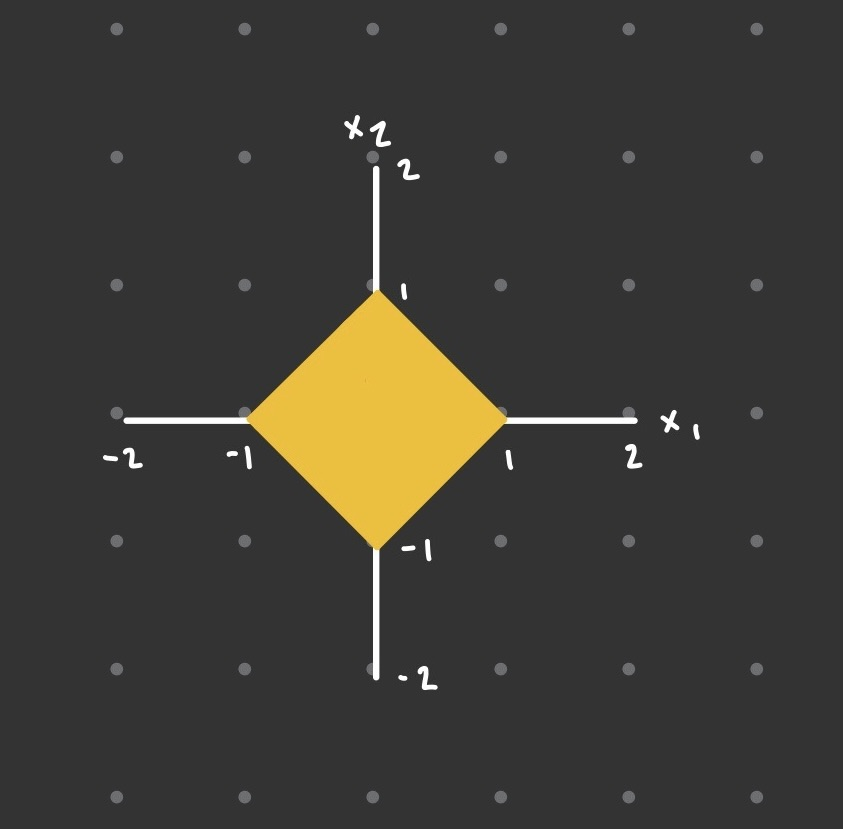
\includegraphics[width=0.4\textwidth]{plots/l1_norm.jpeg} 
	        \captionsetup{labelformat=empty}
	        \caption{}
	        \label{fig:l1_norm}
	    \end{figure}
	\end{soln}
		
		\item 	$||\mathbf{x}||_2 \leq 1$ (Recall that $||\mathbf{x}||_2 =\sqrt{\sum_i x_i^2}$)
			\begin{soln}
			\begin{figure}[h!]
			    \centering
			    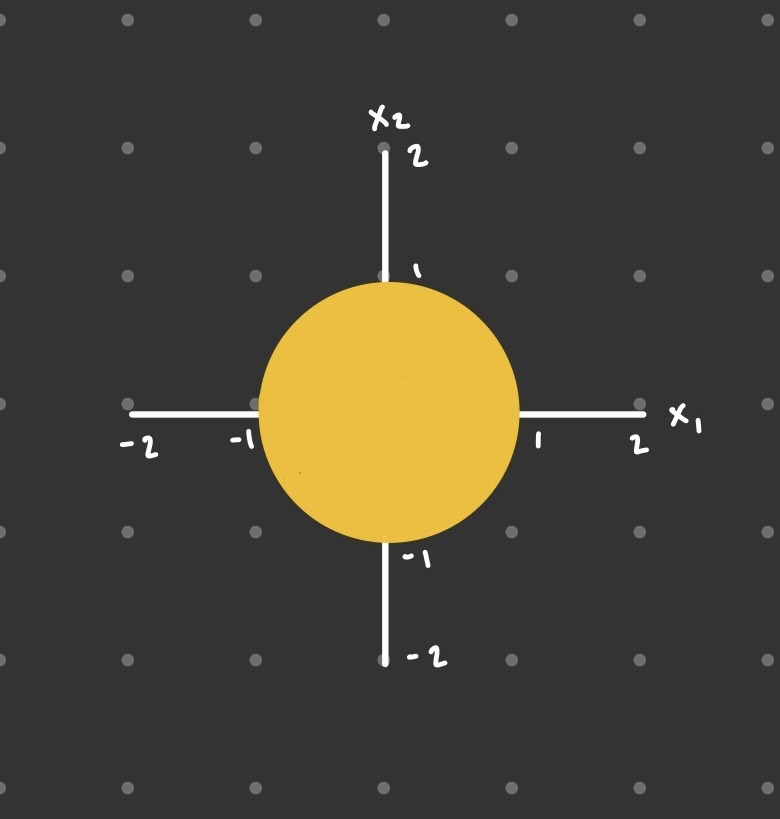
\includegraphics[width=0.4\textwidth]{plots/l2_norm.jpeg}
			    \captionsetup{labelformat=empty}
			    \caption{}
			    \label{fig:l2_norm}
			\end{figure}
		\end{soln}
		\item 	$||\mathbf{x}||_\infty \leq 1$ (Recall that $||\mathbf{x}||_\infty = \max_i |x_i|$)
			\begin{soln}
			\begin{figure}[h!]
			    \centering
			    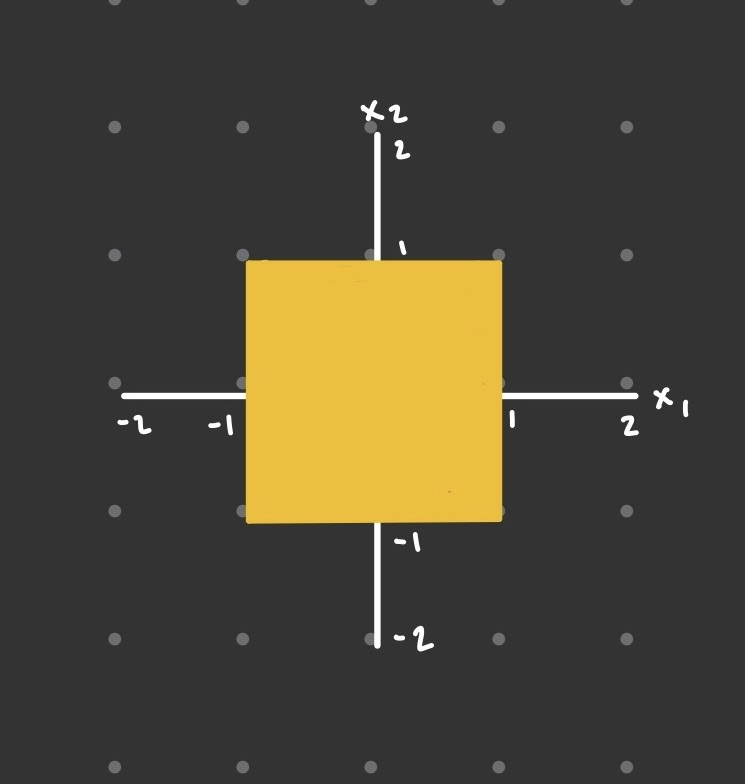
\includegraphics[width=0.4\textwidth]{plots/linf_norm.jpeg}
			    \captionsetup{labelformat=empty}
			    \caption{}
			    \label{fig:inf_norm}
			\end{figure}
		\end{soln}
	\end{enumerate}
	
	For $M = \begin{pmatrix}
		5 & 0 & 0 \\ 0 & 7 & 0 \\ 0 & 0 & 3
		
	\end{pmatrix}$, Calculate the following norms.
	\begin{enumerate}\addtocounter{enumi}{3}
		\item $||M||_{2}$ (L2 norm) \\
		\begin{soln} $||M||_{2} = \sqrt{\lambda_{max}(M^T M)}= 7$ \end{soln}
		
		\item $||M||_{F}$ (Frobenius norm)\\
		\begin{soln} $||M||_{F} = \sqrt{\text{trace}(M^T M)} = \sqrt{83} \approx 9.11$ \end{soln}
		
		
	\end{enumerate}
	
	
	\subsection{Geometry [10 pts]}
	Prove the following.  Provide all steps.
	\begin{enumerate}
		\item 	The smallest Euclidean distance from the origin to some point $\mathbf{x}$ in the hyperplane $\mathbf{w}^{T}\mathbf{x} + b = 0$ is $\frac{|b|}{||\mathbf{w}||_2}$.  You may assume $\mathbf{w} \neq 0$.\\
		\begin{soln}
			Let $x$ be any point in the hyperplane. 
			Because $w$ is orthogonal to the hyperplane, projecting $z$ onto $w$ will give a vector orthogonal to the hyperplane pointing from the origin to a point on the hyperplane, the length of this vector will be the smallest distance to the hyperplane.
			Let $v$ be such vector.
			Then, $v = \frac{x \cdot w}{w \cdot w} w = \frac{-b}{w \cdot w} w$.
			Let $d$ be the smallest distance from the origin to a point on the hyperplane.
			Then, $d = ||v||_2 = \frac{|b| ||w||_2}{||w||_2^{2}} = \frac{|b|}{||w||_2}$.
		\end{soln}
		
		\item 	The Euclidean distance between two parallel hyperplane $\mathbf{w}^{T}\mathbf{x} + b_1 = 0$ and $\mathbf{w}^{T}\mathbf{x} + b_2 = 0$ is $\frac{|b_1 - b_2|}{||\mathbf{w}||_2}$ (Hint: you can use the result from the last question to help you prove this one).\\
		\begin{soln}
			Since both hyperplanes are orthogonal to $w$, the distance between them is equivalent to the distances between the points closest to the origin.
			From above, we know the distance from the hyperplanes to the origin are $\frac{|b_i|}{||w||_2}$ where $i = 1,2$.
			Finally, we either subtract the distances if the hyperplanes are in the same direction or add them if they are in opposite directions from the origin, which is equivalent to $\frac{|b_1 - b_2|}{||w||_2}$.
		\end{soln}
		
	\end{enumerate}
	
	
	
	\section{Programming Skills [10 pts]}
	Sampling from a distribution.  For each question, submit a scatter plot (you will have 2 plots in total).  Make sure the axes for all plots have the same ranges.
	\begin{enumerate}
		\item Make a scatter plot by drawing 100 items from a two dimensional Gaussian $N((1, -1)^{T}, 2I)$, where I is an identity matrix in $\mathbb{R}^{2 \times 2}$.
		
			\begin{soln}
			\begin{figure}[h!]
			    \centering
			    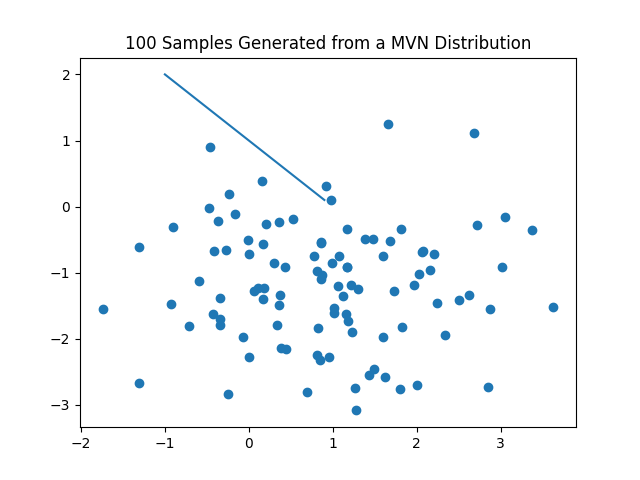
\includegraphics[width=0.8\textwidth]{plots/mvn_samples.png}  
			    \captionsetup{labelformat=empty}
			    \caption{}
			    \label{fig:mvn_samples}
			\end{figure}
		\end{soln}
	
		\item Make a scatter plot by drawing 100 items from a mixture distribution 
		$0.3 N\left((5, 0)^{T}, \begin{pmatrix} 1 & 0.25 \\ 0.25 & 1\\ \end{pmatrix}\right)
		+0.7 N\left((-5, 0)^{T}, \begin{pmatrix} 1 & -0.25 \\ -0.25 & 1\\ \end{pmatrix}\right)
		$.
		
		\begin{soln}
		\begin{figure}[h!]
		    \centering
		    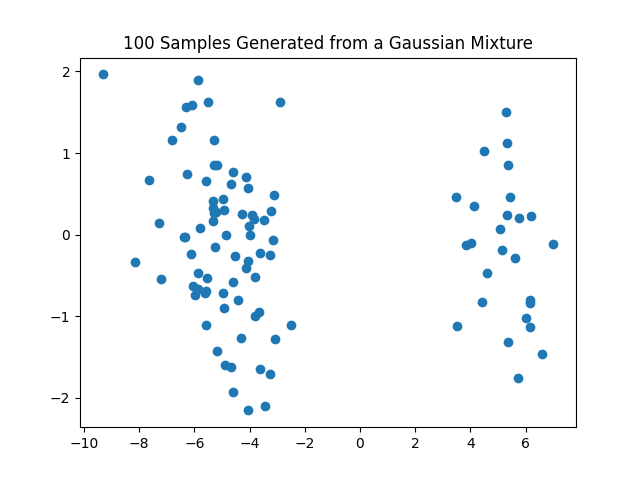
\includegraphics[width=0.8\textwidth]{plots/gm_samples.png}  
		    \captionsetup{labelformat=empty}
		    \caption{}
		    \label{fig:gm_samples}
		\end{figure}
	\end{soln}
	\end{enumerate}
	
	
	\bibliographystyle{apalike}
	
	
	%----------------------------------------------------------------------------------------
	
	
\end{document}
